% Author: Dun-Ming Huang
% Email: dunmingbrandonhuang@berkeley.edu
% CSM16A Fall 2022
%Code references works on https://tex.stackexchange.com/questions/348609/draw-a-3d-sphere-with-radius-with-tikz

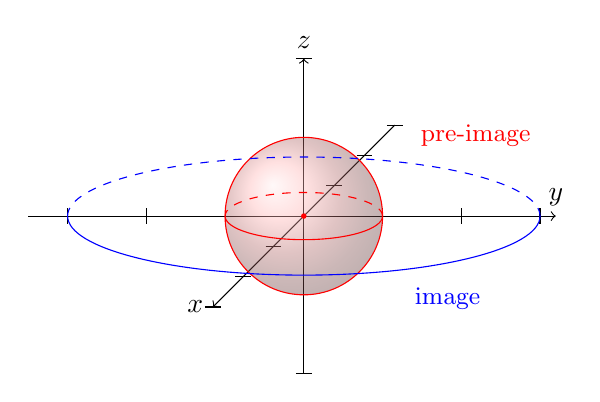
\begin{tikzpicture}
    % Axes
    \draw [->] (0,0,-3) -- (0,0,3) node [left] {$x$};
    \draw [->] (-3.5,0,0) -- (3.2,0,0) node [above] {$y$};
    \draw [->] (0,-2,0) -- (0,0,0) -- (0,2,0) node [above] {$z$};
    
    % Ticks
        \foreach \i in {-3, -2, -1, 1,2,3}
    {
    \draw (\i,-0.1,0) -- ++ (0,0.2,0);
    \draw (-0.1,0,\i) -- ++ (0.2,0,0);
    }
        \foreach \i in {1, 2}
    {
        \draw (-0.1,\i,0) -- ++ (0.2,0,0);
        \draw (-0.1,-\i,0) -- ++ (0.2,0,0);
    }
    
    % Sphere
    \shade[ball color = red!40, opacity = 0.4] (0,0) circle (1cm);
    \draw[draw=red] (0,0) circle (1cm);
    \draw[draw=red] (-1,0) arc (180:360:1 and 0.3);
    \draw[dashed, draw=red] (1,0) arc (0:180:1 and 0.3);
    \fill[fill=red] (0,0) circle (1pt);
    \draw[draw=blue] (-3,0) arc (180:360:3 and 0.75);
    \draw[dashed, draw=blue] (3,0) arc (0:180:3 and 0.75);
    
    % labels
    \node [below right, label={[font=\small,text=red]30:pre-image}] at (1.5,1.2,1) {};
    \node [below right, label={[font=\small,text=blue]30:image}] at (1.5,-0.8, 1.2) {};
    
\end{tikzpicture}